 \documentclass{beamer}

\newlength{\wideitemsep}
\setlength{\wideitemsep}{\itemsep}
\addtolength{\wideitemsep}{10pt}
\let\olditem\item
\renewcommand{\item}{\setlength{\itemsep}{\wideitemsep}\olditem}

\usepackage[utf8]{inputenc}
\usepackage[russian]{babel}
\usepackage{cmap}

\mode<presentation> {
\usetheme{Madrid}
\setbeamertemplate{caption}[numbered]
}

\usepackage{graphicx} % Allows including images
\usepackage{booktabs} % Allows the use of \toprule, \midrule and \bottomrule in tables

\title[Технологии разработки ПО]{Kormushka:\\финансовый микроменеджмент}

\author{Black team.}
\institute[СПб ПУ]
{
Санкт-Петербургский государственный политехнический университет \\
\medskip
\textit{https://github.com/SemenMartynov/kormushka}
}
\date{\today}

\begin{document}

\begin{frame}
\titlepage
\end{frame}

\begin{frame}
\frametitle{Содержание}
\tableofcontents
\end{frame}

%------------------------------------------------
\section{Команда}
%------------------------------------------------

\begin{frame}
\frametitle{Команда: распределение ролей}

\begin{itemize}
\item Мяснов Александр (Client),
\bigskip
\bigskip
\item Дедков Сергей (Project Manager),
\medskip
\item Антон Абрамов (Lead programmer),
\medskip
\item Влад Бусаров (Software Engineer),
\medskip
\item Николай Патраков (Software Engineer),
\medskip
\item Семён Мартынов (Quality Assurance).
\end{itemize}

\end{frame}

%------------------------------------------------
\section{Задача}
%------------------------------------------------

\begin{frame}
\frametitle{О проекте}

\begin{figure}
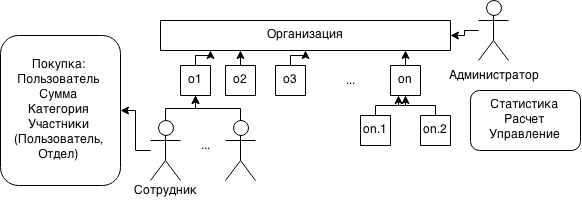
\includegraphics[scale=0.35]{res/r2_about}
\caption{Обзор проекта}
\end{figure}

Основные особенности:
\begin{itemize}
\item Интеграция с LDAP
\item Подробная статистика
\item Web-интерфейс
\item Управление с мобильного телефона
\end{itemize}

\end{frame}

%------------------------------------------------
\section{Задачи второго спринта}
%------------------------------------------------

\begin{frame}
\frametitle{Список задач второго спринта и их статус}

На второй спринт ставились следующие задачи:
\begin{itemize}
\item Мобильный клиент (Android) -- реализована работа по REST API, работа над интерфейсом в процессе.
\item Построение красивых графиков статистики -- нет
\item Полное покрытие тестами -- нет
\item Автоматически генерируемая документация -- нет
\item Deb и (возможно) rpm пакеты с нашим приложением -- да (deb)
\end{itemize}

Решенные задачи, которые не объявлялись на текущий спринт:
\begin{itemize}
\item LDAP -- реализована частичная синхронизация и аутентификация.
\item Доработка функциональности приложения
\end{itemize}

\end{frame}

%------------------------------------------------


\begin{frame}
\frametitle{Основные блоккеры}

Основные проблемы, с которыми мы встретились:
\begin{itemize}
\item Один из участиков команды проболел три недели.
\item Большой объем задач нынешнего семестра.
\end{itemize}


\end{frame}

%------------------------------------------------
\section{Общение с заказчиком}
%------------------------------------------------

\begin{frame}
\frametitle{Общение с заказчиком}

С заказчиком за время спринта встреч не проводилось, т.к. на данный момент фронт работ понятен и вопросов не возникает.

\end{frame}

%------------------------------------------------
\section{Статистика использования СКВ}
%------------------------------------------------

\begin{frame}
\frametitle{Статистика использования СКВ}

\begin{figure}
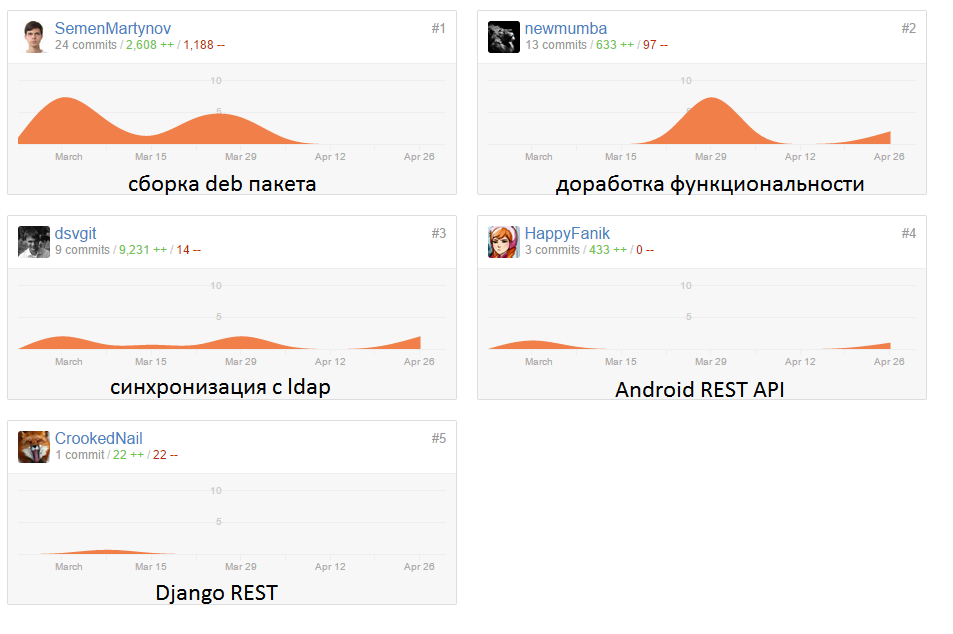
\includegraphics[scale=0.47]{res/r3_stat}
\end{figure}

\end{frame}

%------------------------------------------------
\section{Демонстрация результатов}
%------------------------------------------------

\begin{frame}
\frametitle{Демонстрация результатов}

\begin{figure}[h!]
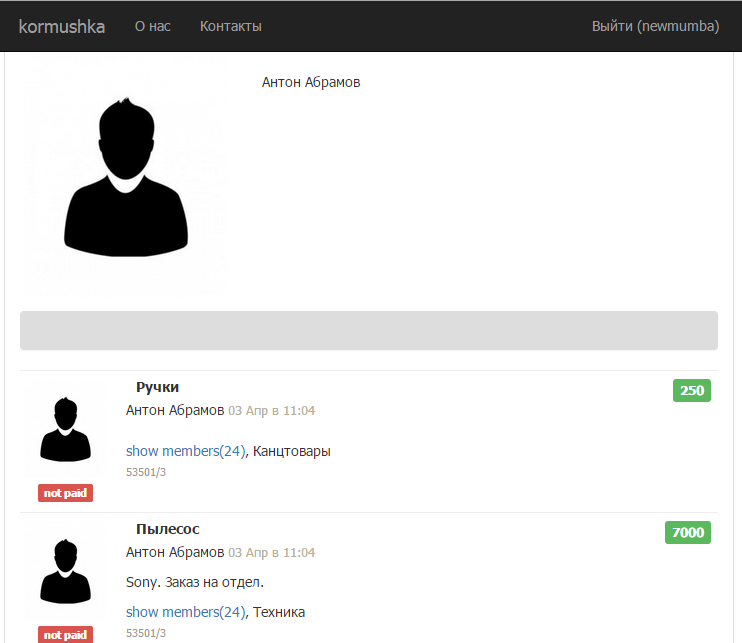
\includegraphics[scale=0.40]{res/r2_result}
\caption{Пример программы}
\end{figure}

\end{frame}

%------------------------------------------------
\section{Цели третьего спринта}
%------------------------------------------------

\begin{frame}
\frametitle{План третьего спринта}

К концу третьего спринта мы достигнем следующих результатов:
\medskip
\begin{itemize}
\item Мобильный клиент (Android)
\item Завершение работы над модулем статистики
\item Завершение работы над тестами и генерацией документации
\item Доработка LDAP
\item Свести все бранчи в master
\end{itemize}

\end{frame}

%------------------------------------------------
\section{Вопросы}
%------------------------------------------------

\begin{frame}
\Huge{\centerline{Вопросы?}}
\end{frame}

%----------------------------------------------------------------------------------------

\end{document} 
